\section{SPO Initialization}
We show the SPO initialization procedure in Algorithm~\ref{alg:SPO-init}.
In the experiments, we use $n_0 = 8$ to have a good estimation of initial baseline tracker. We ablate the setting where we use \emph{no offline estimation} and rely on the online moving estimator in Section~\ref{appendix:ablation}.


\begin{algorithm}[h]
\caption{SPO Initialization}
\label{alg:SPO-init} %
\begin{algorithmic}[1]
\State Set initial effective sample size $N_0 = 1 / (1 - \rho_{\min})$.
\For{each prompt $x \in \mathcal{X}$}
    \State Collect $n_0$ outcomes $\{r^{(k)}\}_{k=1}^{n_0}$ with an initial policy $\pi_0$.
    \State Compute initial value estimate $\hat{v}_{0}(x) = \frac{1}{n_0} \sum_{k=1}^{n_0} r^{(k)}$.
    \State Set $\alpha_0(x) = N_0 \cdot \hat{v}_{0}(x)$ and $\beta_0(x) = N_0 \cdot (1 - \hat{v}_{0}(x))$.
\EndFor
\end{algorithmic}
\end{algorithm}

Practically, one may concern about the extra cost during the offline estimation of $\hat{v}_0$. We note that we share the offline estimation for our experiments so that people could skip this process and directly load our datasets, and there are datasets like Polaris~\cite{Polaris2025} that pre-compute accuracy for Deepseek-R1-Distill-Qwen-7B~\cite{R1}. The cost can be \emph{amortized} across the experiments people run themselves, and we will share more \texttt{(dataset, base\_model)} combinations to facilitate experiment efficiency.


\section{Batch Extensions}
We could adapt Single-stream Policy Optimization (SPO) into a prompt-repetition scheme\footnote{Batch SPO or BSPO}, processing each prompt $G$ times per batch with a shared baseline estimator $\hat{v}$ to better handle sparse rewards. Our method's primary advantage over GRPO lies in its asynchronous nature, achieved by removing the group synchronization barrier. Treating repeated prompts as independent trajectories unlocks two key efficiency improvements. First, it enables robust handling of long-tail generation issues, as slow or problematic trajectories can be terminated early, discarded, or managed via partial rollouts~\cite{team2025kimi} without delaying the entire batch. Second, it facilitates a more flexible batching strategy. By over-sampling the number of initial prompts (e.g., by 50\%), a full training batch can be assembled from the first-finishing trajectories, allowing the optimization step to proceed immediately without waiting for stragglers. This design significantly reduces training latency compared to the rigid group synchronization required by GRPO. When tackling hard prompts, the batch extensions may help obtain learning signals more quickly.

\section{Comparisons against GRPO}\label{appendix:advanatages_over_GRPO}

\subsection{Inefficiency of Dynamic Sampling} 
To address the information loss from degenerate sample groups (where all rewards are identical), methods like DAPO~\cite{DAPO} employ \textit{dynamic sampling}. This strategy continues generating responses for a prompt until the collected set contains at least one success and one failure, guaranteeing a non-zero advantage. While effective at ensuring a learning signal, this approach can be extremely data- and time-inefficient. Note that when people report performance with dynamic sampling, the ``steps'' indicate the \emph{learning} steps rather than the \emph{sampling} steps, where the latter is normally a multiple of the former (e.g., $5\times$).

We can formalize the expected computational cost. For a prompt $x$ with true success probability $p = V_\pi(x)$, let $N$ be the number of samples required to obtain a non-degenerate set. We have:
\[
\mathbb{E}[N \mid p] 
= p\Bigl(1 + \tfrac{1}{1-p}\Bigr) + (1-p)\Bigl(1 + \tfrac{1}{p}\Bigr)
= \frac{1}{p(1-p)} - 1.
\]
This cost grows hyperbolically as the policy becomes either proficient ($p \to 1$) or incompetent ($p \to 0$). For example, if a policy has a 10\% success rate ($p=0.1$), the expected number of generations needed to collect both a success and a failure is $\mathbb{E}[N] \approx 10.11$. In contrast, SPO requires exactly one sample per prompt and uses its adaptive curriculum to actively \textit{de-prioritize} these inefficient prompts, allocating resources to where learning is most effective. This makes SPO fundamentally more scalable and computationally efficient.



\subsection{Variance Reduction for Policy Gradient}

The per-sample policy gradient is $g = A(x,y) \nabla_\theta \log \pi_\theta(y|x)$, where the advantage $A$ is an estimate of the expected return over a baseline. The variance of this gradient, $\mathrm{Var}[g]$, is a key driver of training efficiency. We analyze how the construction of the advantage $A$ leads to significant variance differences between GRPO and SPO.

\textbf{GRPO's High-Variance Group-Based Advantage}: 
GRPO computes advantages by comparing outcomes within a small group of $G$ ($G = 8, 16, ...$) samples generated for the same prompt. The normalized advantage for sample $x$ with binary reward $r \in \{0,1\}$ is
$    \tilde{A}_{\text{GRPO}} = \frac{r - \mu_\mathcal{G}}{\sigma_{\mathcal{G}} + \epsilon}$,
where both the baseline $\mu_\mathcal{G}$ (e.g., the group mean $\frac{1}{G}\sum_{j} r_j$) and the standard deviation $\sigma_{\mathcal{G}}$ are estimated from the same small group of $G$ samples. This coupled, small-sample estimation introduces three fundamental sources of variance:
\begin{itemize}
    \item \textbf{Noisy Baseline (Numerator):} The baseline $\mu_\mathcal{G}$, estimated from only $G$ samples, where $G$ is small, is a high-variance quantity. This inflates the variance of the unnormalized advantage $(r - \mu_\mathcal{G})$ by a factor of $(1 + \frac{1}{G})$ compared to using an optimal baseline.
    \item \textbf{Noisy Scaling (Denominator):} The standard deviation $\sigma_{\mathcal{G}}$, estimated from only $G$ samples, is also highly variable. Scaling the gradient by this noisy random variable further increases total variance.
    \item \textbf{Information Loss (Degeneracy):} When all rewards in the group are identical (e.g., all 0s or all 1s), the advantage for every sample becomes zero, providing no gradient signal. This event, which occurs with probability $Z_G(p) = p^G + (1-p)^G$ where $p=V^\pi(x)$, effectively reduces the batch size and inflates variance by a factor of $1/(1-Z_G(p))$, an issue that is especially severe for easy ($p \approx 1$) or hard ($p \approx 0$) prompts.
\end{itemize}

\textbf{SPO's Low-Variance Decoupled Advantage}:
In contrast, SPO is designed to minimize these variance sources by decoupling the advantage calculation from the current group of samples. It uses an action-independent baseline $b = \hat{v}(x)$ from a historical tracker, which provides a stable, low-variance estimate of the true success probability $p$. The advantage is simply $A_{\text{SPO}} = \texttt{batch\_norm}(r(x, y) - \hat{v}(x))$. Crucially, SPO then applies \emph{global} normalization~\cite{PPO,andrychowicz2020matters,liu2025part}, scaling all advantages in a large batch of size $B \gg G$ by a single, stable standard deviation $\sigma_{\text{batch}}$. This design avoids GRPO's pitfalls: the baseline $b$ is near-optimal, the normalization scaler $\sigma$ is stable, and there is no systematic information loss from group-outcome degeneracy.



\textbf{Quantitative Comparison}: A simplified ratio of the reward-term variance quantifies the difference:
\begin{equation}
\frac{\text{Var}[g]_{\text{GRPO}}}{\text{Var}[g]_{\text{SPO}}} \approx \underbrace{\frac{1 + \frac{1}{G}}{1 + \frac{1}{N_{\text{eff}}+1}}}_{\text{Baseline Noise}} \times \underbrace{\frac{1}{1 - Z_G(p)}}_{\text{Information Loss}} \times \underbrace{\frac{1 + \psi_G}{1 + \psi_{\mathcal{B}}}}_{\text{Normalization Noise}}.
\end{equation}
Here, $N_{\text{eff}}$ is the effective sample count for SPO's tracker, and $\psi_G > 0$ captures the excess variance from per-group, $\psi_\mathcal{B}$ represents the excess variance introduced by estimating the normalization statistics (mean and standard deviation) from a large global batch of size $N_\mathcal{B}$ ($\psi_\mathcal{B} \approx 0$). For a moderately difficult prompt ($p=0.5$) with $G=8$, the normalization noise dominates. However, for an easy/hard prompt ($p=0.9 / p=0.1$), the information loss term dominates, and the ratio swells to $\approx 1.97$. While increasing $G$ in GRPO mitigates information loss, it does so at a multiple generation cost and cannot fix the inherent noise from its small-sample baseline and scaling. SPO achieves lower variance more efficiently by design.




\section{Training and Evaluation Details}
\label{appendix:training_details}
All experiments in this paper are implemented on top of verl~\cite{verl} and ReTool~\cite{feng2025retool} for the tool-integrated reasoning setup.
During training, we set the maximum response length to $16{,}384$ tokens. 
The policy learning rate is fixed at $1\times 10^{-6}$. 
Following DAPO~\cite{DAPO}, we adopt the Clip-Higher mechanism, with clipping parameters $\varepsilon_\text{low}=0.2$ and $\varepsilon_\text{high}=0.28$, to balance exploration and exploitation. 
The sampling parameters are set to temperature 1.0, top-$p =1.0$, and top-$k=-1$.
The forgetting rate thresholds are chosen as $\rho_{\min} = 0.875$ and $\rho_{\max} = 0.96$, yielding window sizes $W_{\min} = 1 - \tfrac{1}{\rho_{\min}} = 8$ and $W_{\max} = 25$.

GRPO rollouts are collected with multiple responses per prompt, and training mini-batch sizes are chosen such that $8$ gradient updates are performed per rollout step. 
For a fair comparison, the prompt batch size in SPO is set equal to the total number of responses in GRPO, as SPO generates only a single response for each prompt. Specifically, GRPO uses a prompt batch size of $256$ with $8$ responses per prompt and a training mini-batch size of $256$, while SPO operates on $2,048 = 256 \times 8$ prompts. Both algorithms are set with maximum of $8$ Python interpreter interaction turns.

For evaluation on hard math competition benchmarks, i.e., AIME 24, AIME 25, BeyondAIME~\cite{seed1.5}, BRUMO 25~\cite{matharena} and HMMT 25~\cite{matharena}, we set sampling parameters to temperature $0.6$, top-$p$ $0.95$, and top-$k$ $20$, as officially recommended\footnote{https://huggingface.co/Qwen/Qwen3-8B}.
We define a binary reward function $r_{i,j}$ such that a response receives $r_{i,j}=1$ if the final answer is correct, and $r_{i,j}=0$ otherwise.
The same reward function is consistently used during training for policy optimization and during evaluation. We set the maximum response token to 32,768.

Given a test set with $M$ problems, and for each problem $i$ we independently sample $k$ responses with rewards $\{ r_{i,1}, r_{i,2}, \ldots, r_{i,k} \}$, we define:

\begin{itemize}
    \item \textbf{avg@}$k$: the expected correctness of an individual response:
    \[
        \text{avg@}k = \frac{1}{M} \sum_{i=1}^{M} \frac{1}{k} \sum_{j=1}^{k} r_{i,j}.
    \]
    \item \textbf{pass@}$k$: the probability of solving a problem within $k$ attempts. 
    Directly computing $\mathbf{1}\!\bigl(\max_{1 \leq j \leq k} r_{i,j}=1\bigr)$ can lead to high variance.
    Following~\cite{chen2021evaluating}, we instead generate $n \geq k$ responses per problem, count the number of correct ones $c \leq n$, and use the unbiased estimator:
    \[
        \text{pass@}k = \frac{1}{M} \sum_{i=1}^{M} \left[ 1 - \frac{\binom{n-c_i}{k}}{\binom{n}{k}} \right],
    \]
    where $c_i$ denotes the number of correct responses for problem $i$.
    \item \textbf{maj@}$k$: the correctness of the majority-voted answer~\cite{maj}. This metric first identifies the most frequent answer among $k$ responses for each problem. The score is 1 if that modal answer is correct, and 0 otherwise. Let $a_{i,j}$ be the final answer string for the $j$-th response to problem $i$, and let $r(\cdot)$ be the reward function for a given answer string. The metric is defined as:
    \[
        \text{maj@}k = \frac{1}{M} \sum_{i=1}^{M} r\left(\operatorname{mode}\{a_{i,j}\}_{j=1}^k\right).
    \]
\end{itemize}

\section{Ablation Studies}
\label{appendix:ablation}

We conduct a series of ablation studies to dissect the core components of SPO and validate our design choices. To facilitate efficient experimentation, these studies are performed under a streamlined setting compared to our main experiments. Specifically, we utilize a batch size of $256$ prompt-response pairs, and the model is updated with $4$ gradient steps for each collected batch. All ablation results are reported on the AIME 25 benchmark, using the avg@16 metric with a maximum generation length of $16,384$ tokens.


\begin{figure}[h!]
    \centering
    \begin{adjustbox}{width=0.95\textwidth, center}
    \begin{minipage}{\textwidth}
    \begin{subfigure}{0.31\textwidth}
        \centering
        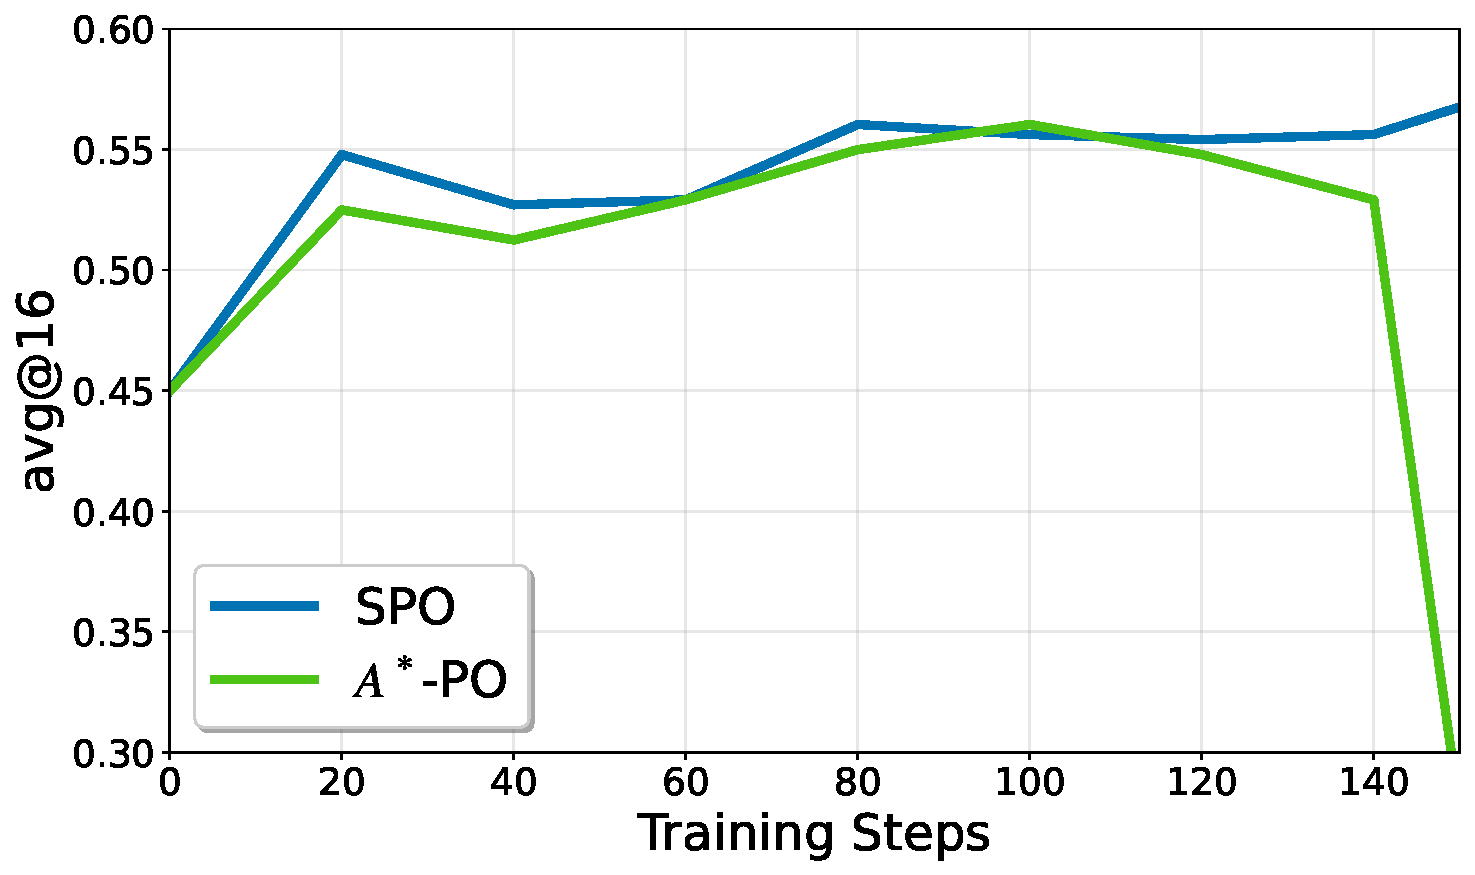
\includegraphics[width=\linewidth]{figures/spo_vs_apo_validation_reward.pdf}
        \caption{SPO \emph{vs.} $A^*$-PO}
        \label{fig:spo_vs_apo}
    \end{subfigure}
    \hfill %
    \begin{subfigure}{0.31\textwidth}
        \centering
        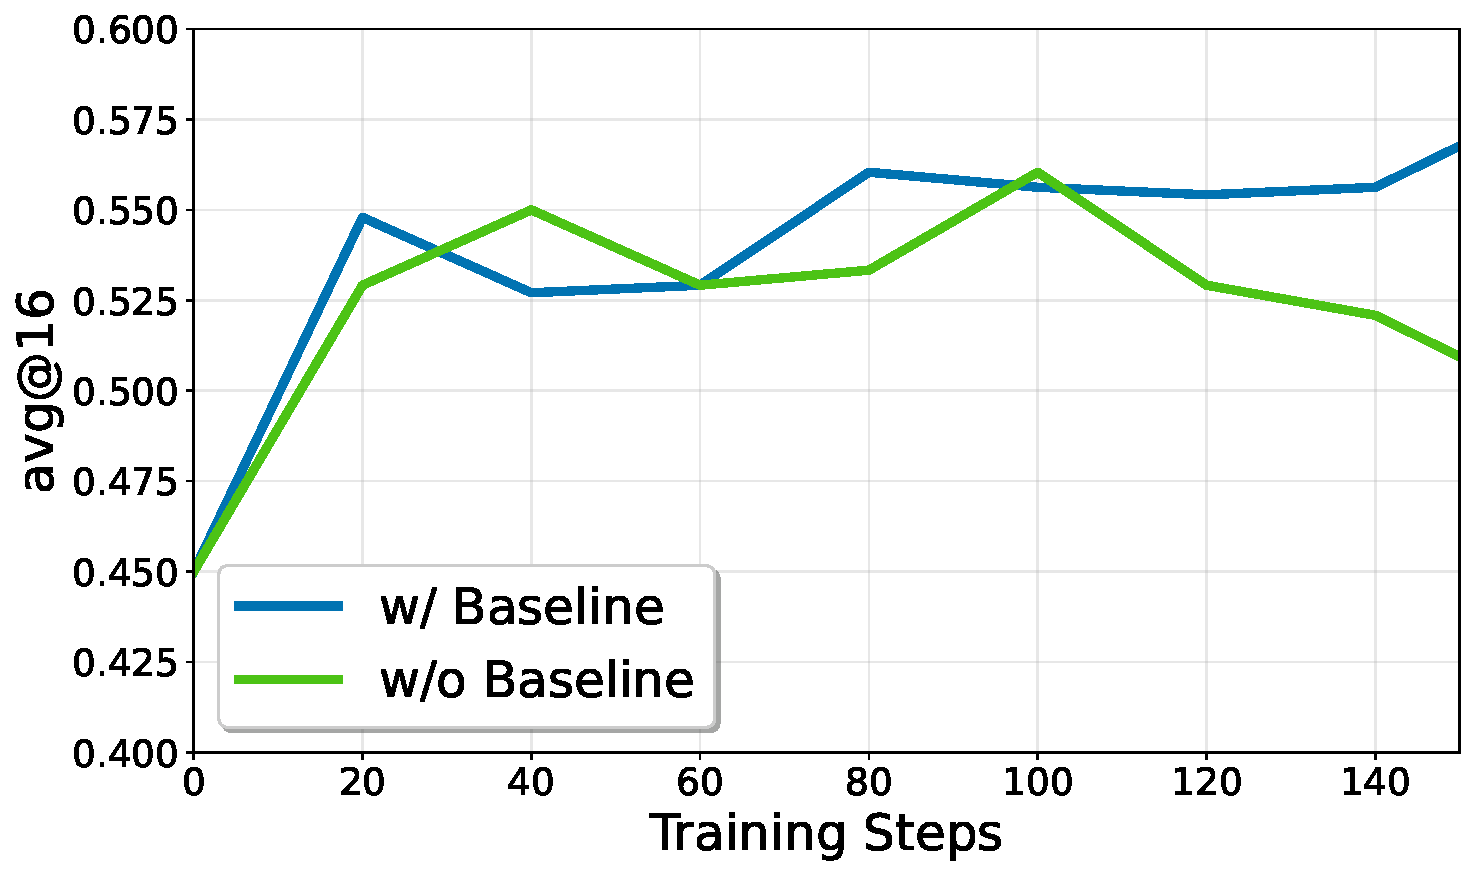
\includegraphics[width=\linewidth]{figures/spo_vs_no_baseline_validation_reward.pdf}
        \caption{Baseline Ablation}
        \label{fig:spo_vs_no_baseline}
    \end{subfigure}
    \hfill %
    \begin{subfigure}{0.31\textwidth}
        \centering
        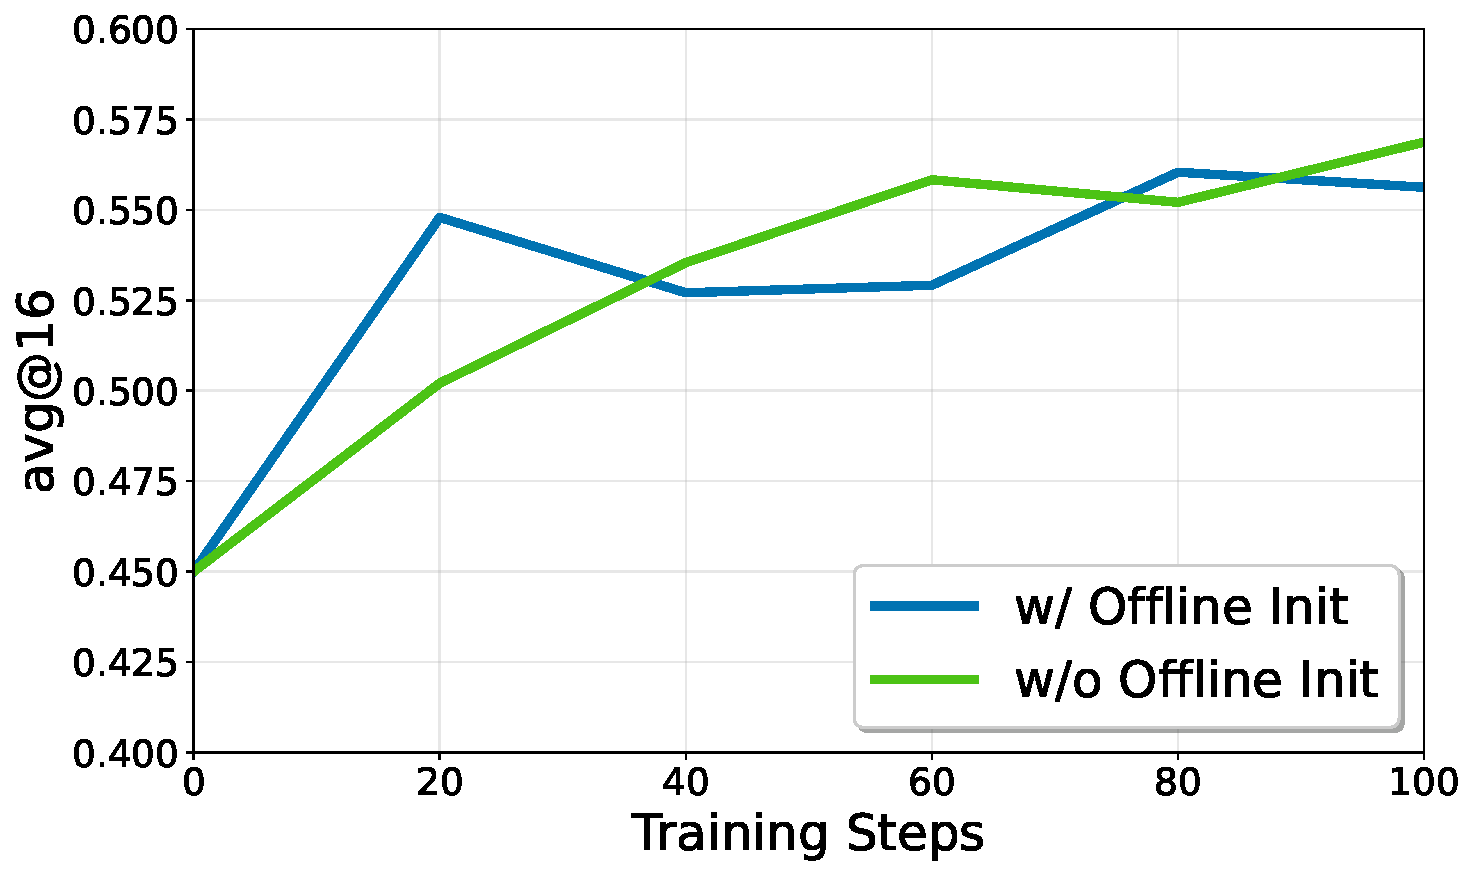
\includegraphics[width=\linewidth]{figures/spo_vs_no_offline_validation_reward.pdf}
        \caption{Offline Initialization Ablation}
        \label{fig:spo_vs_no_offline}
    \end{subfigure}
    \end{minipage}
    \end{adjustbox}
    \caption{Ablation studies evaluating the core components of SPO. (a) SPO's adaptive baseline outperforms the static baseline of $A^*$-PO, demonstrating the benefit of a value function that evolves with the policy. (b) Removing the value tracker (``w/o Baseline'') causes a severe performance drop, confirming its critical role in reducing gradient variance. (c) Eliminating the offline initialization step (``w/o Offline Init'') leads to initial training instability and suboptimal convergence, highlighting the importance of a warm start for the value tracker.}
    \label{fig:ablation_studies}
\end{figure}


\textbf{SPO \emph{vs}. $A^*$-PO}. This experiment, presented in Figure~\ref{fig:spo_vs_apo}, compares our proposed SPO with $A^*$-PO~\cite{brantley2025accelerating}. $A^*$-PO utilizes a static baseline derived from a pre-computed optimal value function, $V^*$, which is tied to the KL-regularized objective with respect to an initial reference policy, $\pi_{\text{ref}}$. While this approach is highly efficient, its central assumption may be challenged in tool-calling scenarios. In these tasks, learning involves acquiring new functional capabilities, leading to a significant policy drift where the learned policy, $\pi_t$, diverges substantially from $\pi_{\text{ref}}$. Consequently, the pre-computed $V^*$ may become a less representative baseline for the current policy's true value function, $V_{\pi_t}$, potentially affecting the accuracy of the advantage estimates. In contrast, SPO's baseline is adaptive, dynamically tracking an estimate of $V_{\pi_t}$ as the policy evolves. The empirical results, which show SPO's superior performance, suggest that this adaptability is crucial. By maintaining a baseline that remains relevant to the current policy, SPO provides a more stable and effective learning signal in environments that demand significant policy evolution. Finally, from a practical perspective, $\pi_\text{ref}$ computation during $A^*$-PO policy update occupies an extra trunk of GPU memory, making it less appealing than the proposed SPO algorithm.

\textbf{Baseline Ablation}. Figure~\ref{fig:spo_vs_no_baseline} presents a crucial ablation that validates the fundamental principle of using a baseline for variance reduction. In this experiment, we remove the value tracker component $\hat{v}_{-1}(x)$ from the advantage calculation, causing the algorithm to rely solely on the globally batch-normalized raw reward $r(x,y)$ as its learning signal. However, the substantial performance degradation observed is a classic illustration of the remaining challenges. While global normalization effectively controls the overall scale of rewards, the raw reward signal is still noisy on a per-sample basis as it fails to account for prompt-specific difficulty. SPO's history-informed baseline is designed to subtract this expected difficulty, thereby effectively reducing variance and providing a much cleaner, more reliable gradient for learning. This experiment confirms that the adaptive value tracker is the most critical component for SPO's success, directly addressing the core challenge of variance in single-stream policy optimization.

\textbf{Offline Initialization Ablation}. In Figure~\ref{fig:spo_vs_no_offline}, we analyze the impact of the value tracker's initialization phase. The standard SPO algorithm initializes the value tracker with estimates computed from a small set of $n_0$ offline samples, giving it a ``warm start''. The ablation removes this step, forcing the tracker to learn from scratch online. The results clearly demonstrate the benefit of the offline initialization. Without it, the tracker begins with a highly inaccurate baseline, leading to high-variance gradients and significant instability in the initial training phase, as evidenced by the performance dip. Although the model eventually recovers, it fails to reach the same level of performance as the properly initialized model, underscoring the importance of a good initial value estimate for stable and effective learning.
